% Chapter 2

\chapter{Theoretical Background} % Main chapter title

\label{Chapter2} % For referencing the chapter elsewhere, use \ref{Chapter2}

%----------------------------------------------------------------------------------------

\section{Significant Wave Height and Wave Spectra}\label{swh_spectra}

Historically, the study of wave growth and the interest in its prediction have their origins in the Second World War when it was critical for landing operations. Munk \cite{Munk2010} classified ocean waves according to their propagation period and documented the need for further comprehension of the wave spectrum. The band of the range of ocean waves that we are focusing on in this study is the ordinary gravity waves, as shown in Figure~\ref{fig:ocean_waves}. Wave characteristics that describe what we call sea state were first observed visually and empirically defined. Since then, a better understanding of the generation of waves and the need for reliable and continuous observations led to what we perceive as the SWH and wave spectrum nowadays.


\begin{figure}[H]
\centering
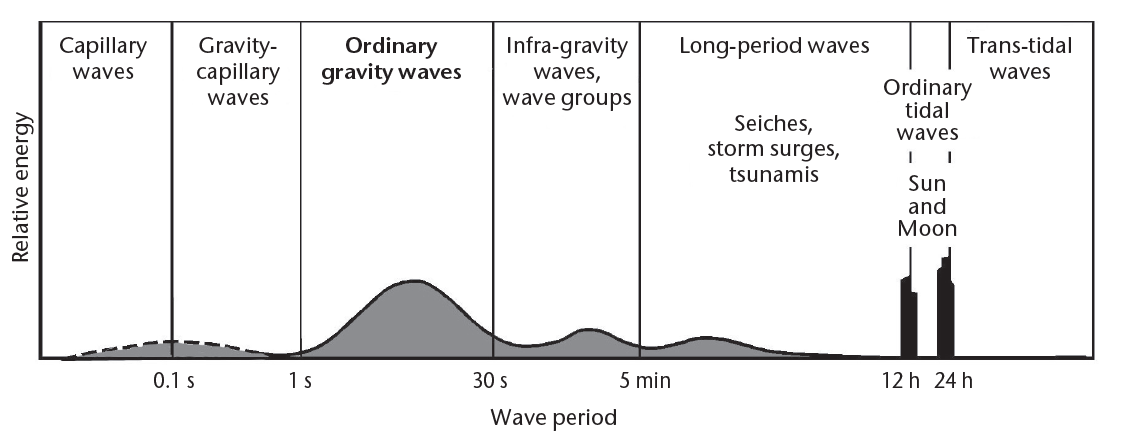
\includegraphics[width=0.95\linewidth]{Figures/Chapter2/ocean_waves.png}
%\decoRule
\caption{The classification of ocean waves depending on their period according to Munk \cite{Munk2010}. Reprinted from: \cite{Organization1998a}}
\label{fig:ocean_waves}
\end{figure}


First, we need to define the linear waves' fundamental parameters. The wavelength \emph{$\lambda$} is the horizontal distance between two consecutive crests of a wave in meters, and it is connected with the wavenumber \emph{k}, the number of crests per unit distance:


\begin{equation}
k = \frac{2\pi}{\lambda}
\label{eqn:wavenumber}
\end{equation}


Wave frequency \emph{f} is equal to the number of crests that pass from a point every second. Wave period \emph{T} is the time interval in seconds between the passage of successive crests from a fixed location. They are both related with the angular frequency \emph{$\omega$} in radians per second:


\begin{equation}
\omega = \frac{2\pi}{T} = 2\pi f
\label{eqn:angular_frequency}
\end{equation}

The wavenumber and wave frequency are connected with the dispersion relation, which characterizes wave propagation variation. The dispersion relation of ordinary gravity waves for specific depth \emph{h} is given by: 

\begin{equation}
\omega^{2} = gk\tanh{kh} 
\label{eqn:dispersion_relation}
\end{equation}

Other important parameters, especially for navigation and offshore installations, include the amplitude $\alpha$, which is the maximum displacement from the mean or zero sea level, and the wave height \emph{H}, which is the vertical distance of the successive troughs and crests, both measured in meters. Finally, we need to know the wave direction in degrees from which the waves propagate to characterize the sea state.

 
The definition of random ocean waves rests on the assumption that they are a superposition of an infinite number of components. Each wave component is characterized by a unique combination of frequency and propagation direction. The vertical displacement of waves in 2-dimensional space and time is given by the sum of the components' surface elevation \cite{Goda2010a}:
 
 \begin{equation}
\eta \left(x, y, t\right) = \sum_{n=1}^{\infty} \alpha_{n} \cos{\left(k_{n}x \cos{\theta_{n}} + k_{n}y \sin{\theta_{n}} - 2\pi f_{n}t + \epsilon_{n}  \right)}
\label{eqn:wave_elevation_3d}
\end{equation}
 
 Each wave component has a different phase angle \emph{$\epsilon_{n}$} between 0 and $2\pi$. The sum of the squared amplitudes of the wave components has a unique value:
 
\begin{equation}
\sum_{f}^{f+df} \sum_{\theta}^{\theta+d\theta} \frac{1}{2} \alpha^{2}_{n} = S\left(f,\theta\right)dfd\theta
\label{eqn:amplitude_spectrum}
\end{equation}
 
The function $S\left(f,\theta\right)$ is the directional wave spectrum, and it represents the wave energy distribution with respect to the different frequencies and directions of ocean waves because the squared amplitudes are also present at the wave energy equation:
 
\begin{equation}
E = \frac{\rho_{w}gH^{2}}{8} = \frac{\rho_{w}g\alpha^{2}}{2} 
\label{eqn:wave_energy}
\end{equation}

Where $p_{w}$ is the water density and \emph{g} is the gravitational acceleration constant. Therefore, a transformation of $S(f,\theta)$ to $p_{w}gS(f,\theta)$ is necessary first to be consistent with the energy spectrum term. The total wave energy is represented by $m_{0}$ which is the zeroth-moment of the spectrum \cite{Ardhuin2019a}, and it is calculated by the integral of the $S(f,\theta)$ function in all frequencies and directions:

\begin{equation}
m_{0} = \int_{0}^{\infty} \int_{0}^{2\pi} S(f,\theta) df d\theta
\label{eqn:total_wave_energy}
\end{equation}

This integral is by definition equal to the surface elevation variance $\overline{\eta^{2}}$. Thus, wave elevation variance is a more accurate term than wave energy. SWH is defined as four times the Root-Mean-Square (RMS) of the elevation variance, and it is denoted as \emph{$H_{s}$} or \emph{$H_{m0}$}.

\begin{equation}
H_{s} = 4\sqrt{m_{0}}
\label{eqn:swh_hs}
\end{equation}
 
 
 
When directional information is unavailable, we can obtain the wave spectrum as a function only of the frequencies. It becomes the frequency spectrum, an example of which is shown in Figure~\ref{fig:freq_spectrum} using buoy observations. The infinite number of wave frequencies are represented on the x-axis. In reality, sensors onboard buoys divide the whole spectrum into frequency bands with an \emph{f+df} size. NDBC uses frequency bands of 0.01 Hz size with a cut-in frequency of 0.03 Hz and a cut-off frequency of 0.4 Hz. On the other hand, CDIP uses narrower frequency bands of 0.005 Hz for a more extended spectrum with a cut-in frequency of 0.025 Hz and a cut-off frequency of 0.58 Hz. The elevation variances or the wave energies are plotted on the y-axis in $m^{2}s$ or $m^{2}/Hz$.


 
\begin{figure}[H]
\centering
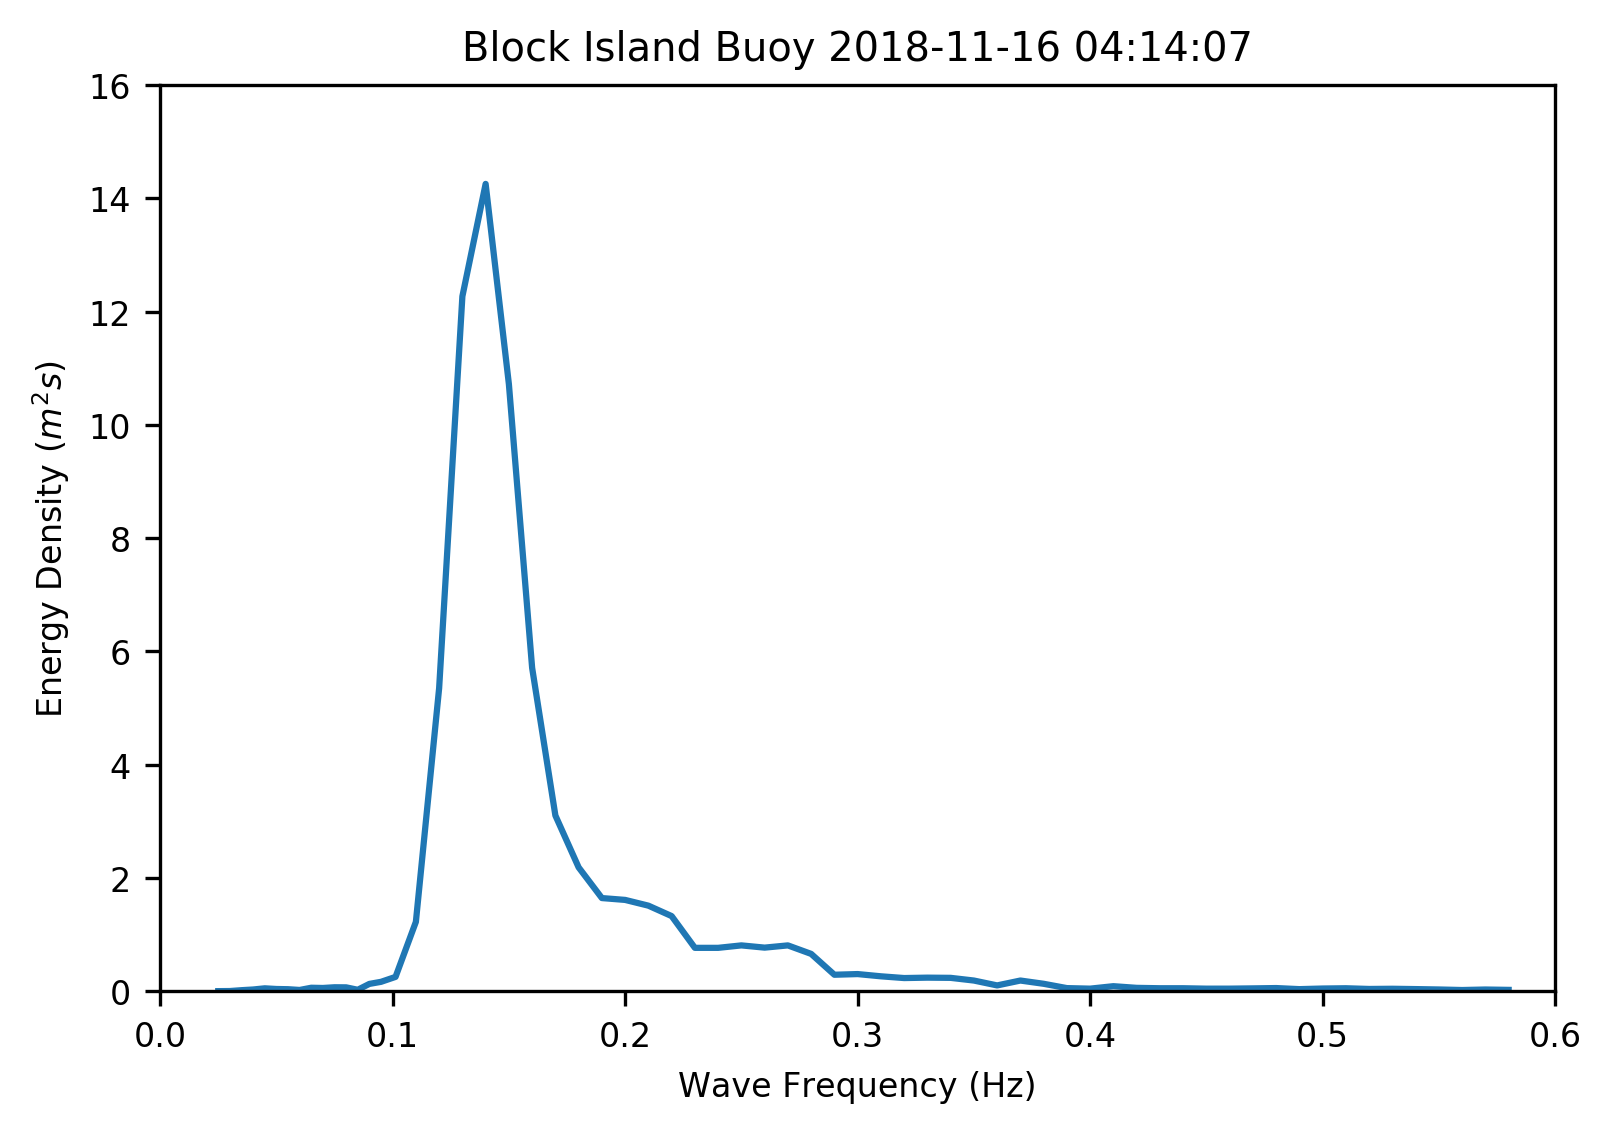
\includegraphics[width=0.85\linewidth]{Figures/Chapter2/freq_spectrum.png}
%\decoRule
\caption{An example of a wave frequency spectrum. Data presented were reported from Block Island buoy 44097 on October 27 2018.}
\label{fig:freq_spectrum}
\end{figure}


From the frequency spectrum, we can derive two primary parameters for our study, the SWH and the peak or dominant period $T_{p}$. The integral of the spectrum that represents the volume of the area under its continuous curve in Figure~\ref{fig:freq_spectrum} is equal to the zeroth-moment of the spectrum $m_{0}$, and it is the representative value of the total wave energy as defined in \ref{eqn:total_wave_energy}. Therefore, SWH is expressed as four times the square root of this integral. From the frequency spectrum, we can also derive the peak frequency $f_{p}$, which is the wave frequency of the spectrum's peak band. The wave dominant period $T_{p}$ corresponds to the peak frequency band.


To estimate SWH and $T_{p}$ from the wave spectrum accurately, observations are assumed to represent statistically stationary random processes. The aim is to prevent scattering of the observation values; hence, we need a relatively large wave measurement record \cite{Organization1998a}. To satisfy both conditions, NDBC and CDIP stations record raw 1 Hz observations for 20 minutes (see \ref{buoy_observations}).


The directional wave spectrum \emph{S(f,$\theta$)} is the distribution of the elevation variance or the wave energy both in the frequency domain and the wave components' direction. An example of the directional wave spectrum from buoy observations is shown in \ref{fig:dir_spectrum} and the wave energy density is reported in $m^{2}s/deg$ or $m^{2}s/rad$.


Except for the SWH and $T_{p}$, we also need information relative to the ocean waves' direction to obtain a complete picture of the sea state. Except for the surface elevation, buoys contain directional wave sensors measuring the slope vector, and they are included in their raw time series. These measuring systems are called heave pitch and roll, and the slope time series are measured in the east-west, and north-south direction using buoy azimuth \cite{Steele1998}. 
 
 
The directional wave spectrum is also expressed as:
 
 \begin{equation}
S(f,\theta) = S(f)D(f,\theta)
\label{eqn:amplitude_freqdir_spectrum2}
\end{equation}

where $D(f,\theta)$ is the directional spreading function:

\begin{equation}
\int_{-\pi}^{\pi} D(f,\theta)d\theta = 1
\label{eqn:directional_spreading}
\end{equation}

\emph{D(f,$\theta$)} describes how the wave energy density is spread in all directions. Longuet-Higgins \cite{longuet1963}, estimated the wave spectrum using the Fourier series methodology and proved that the first four coefficients are needed to describe the spectrum, including its directional parameters. The four Fourier coefficients are calculated by applying cross-spectral analysis to the wave elevation and the buoys' slope time series. This process is extensively described in \citep{Dean1991a, Earle1996, Earle1999, Kuik1988}.

\begin{figure}[H]
\centering
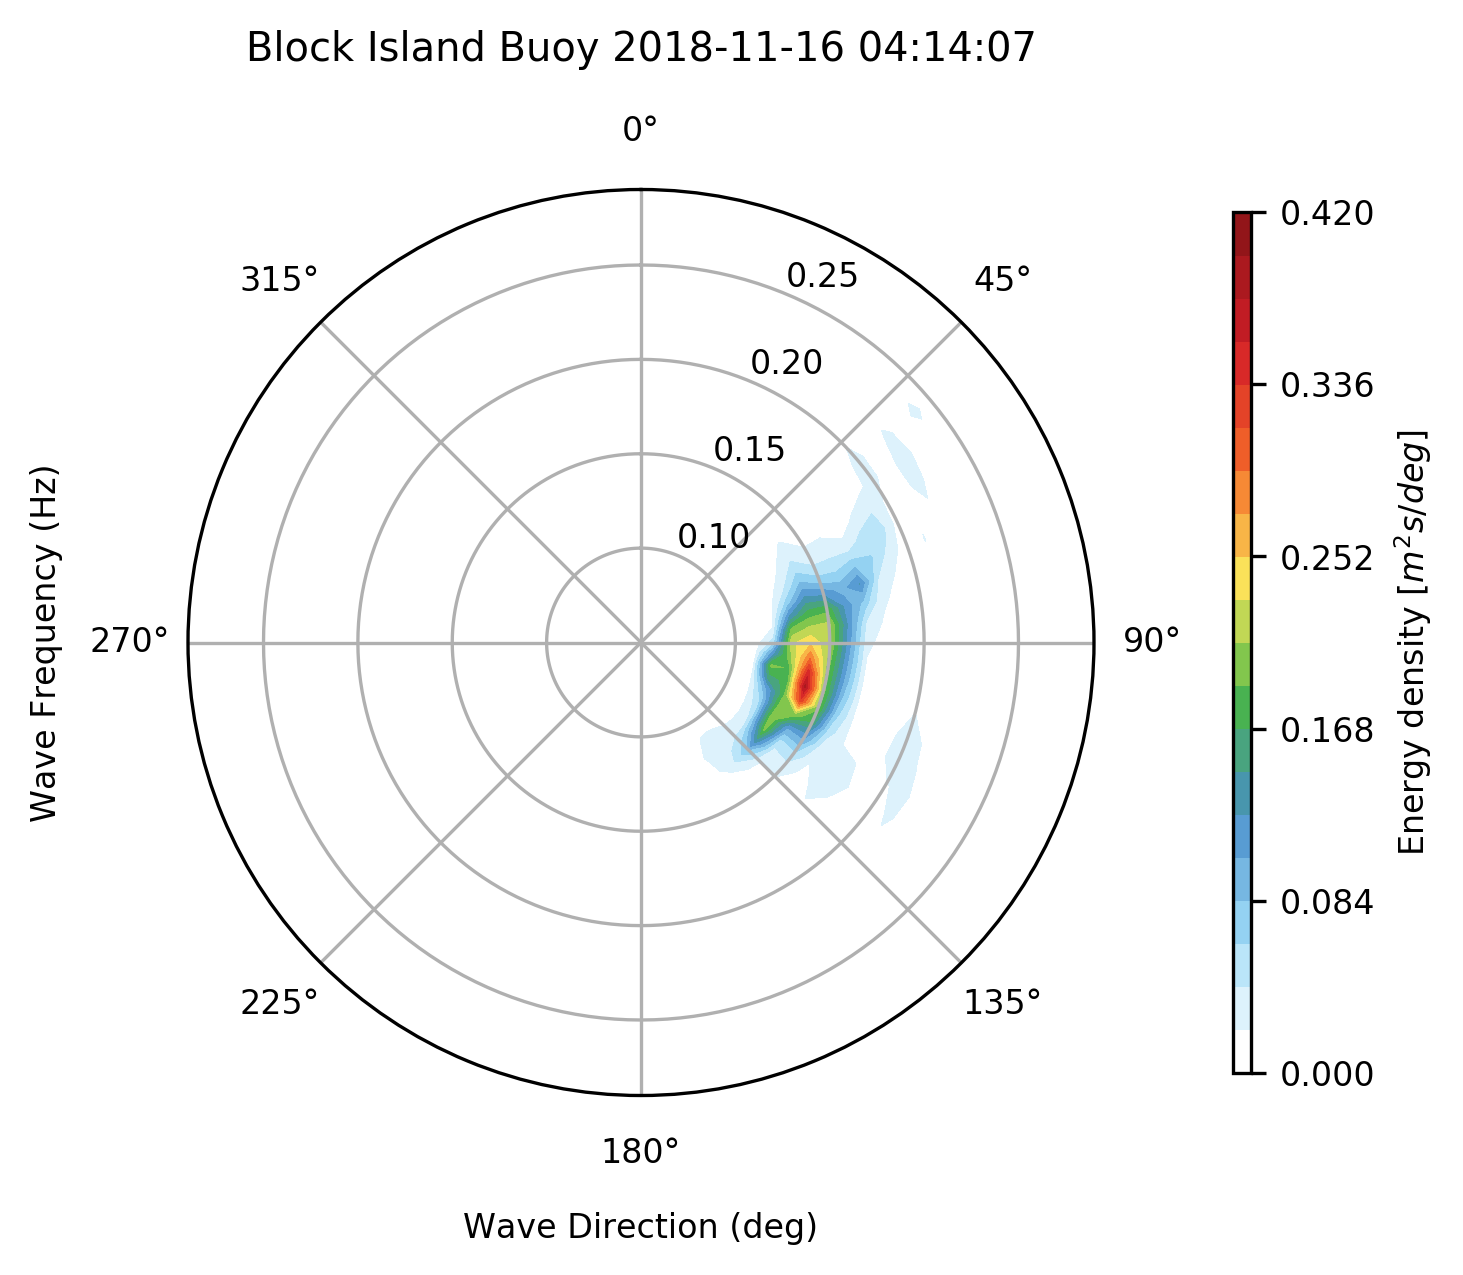
\includegraphics[width=0.85\linewidth]{Figures/Chapter2/dir_spectrum.png}
%\decoRule
\caption{An example of a wave directional spectrum. Data presented were reported from Block Island buoy 44097 for October 27 2018.}
\label{fig:dir_spectrum}
\end{figure}

The challenge is to reconstruct the directional spreading function from the estimated Fourier coefficients and create the directional spectra. It is worth mentioning that NDBC buoys, using the Datawell Hippy 40 sensor, measure and then disseminate the frequency spectrum and the four Fourier coefficient time series \cite{Steele1998}. Still, the final two-dimensional spectra are not provided. CDIP provides only recent directional spectra online. There are several methods to reconstruct the two-dimensional, directional spectra. The Maximum Entropy Method (MEM) \cite{Lygre1986}, is considered the most reliable \cite{Ardhuin2019a}. CDIP also uses this method to reconstruct the directional spectra. Its disadvantage is that often the spectrum's shape contains artificial double-peaks. An extended discussion of the various methods to reconstruct the directional spectrum is available in \cite{Earle1999, Goda2010c, Young1999a}.


%---------------------------------------------------------------------------


\section{Wave Age and Spectral Decomposition}\label{decomposition_waveage}


In the previous section, we discussed the importance of the directional wave spectra to describe the ocean wave conditions. We also emphasized that the waves contributing to the wave spectrum have various frequencies, directions, heights, and periods. This leads us to study waves according to their unique characteristics and influence on the wave climate. 

Waves can be classified according to their growth status. Local waves that owe their development to the increasing momentum input from the wind are called wind waves or wind sea. When the wind speed is reduced, and the wind's relative direction with the waves is increased over 30 degrees, or when remotely-generated waves due to a distant storm arrive, they are called swell \cite{Organization1998a}. Wind waves  are strongly correlated with the wind, and they have a notable presence during extreme events, in enclosed basins, and coastal regions. An empirical method often used is to classify waves as wind sea when their dominant period has a duration of fewer than 10 seconds. In contrast, swells are not coupled with the wind, and they do not owe their development to a local wind momentum input. Besides, swell waves are different visually, as they appear as more organized groups of waves with smoother crests. In this study, we will focus on two methods of ocean wave classification.

The first method is based on ocean waves' growth using the inverse wave age criterion \cite{Hanley2010}. Wave age $c_{p}/U_{10}\cos{\theta_{d}}$ represents the wind's potential to transfer energy to the waves \cite{Zhao2019}. $c_{p}$ is the wave phase speed at the peak of their spectrum and it is equal to $\lambda_{p}/T_{p}$ or $\omega_{p}/k_{p}$. Once wind-waves are generated, the wind is faster than the waves. As the energy is provided to the wind waves, their celerity increases until they reach the wind-wave equilibrium, at which the sea is considered mature or fully developed:


\begin{equation}
\frac{c_{p}}{U_{10}\cos{\theta_{d}}} = 1.2
\label{eqn:wave_age}
\end{equation}

$u_{10}$ is the wind speed at 10 meters height, which is discussed in the next Section~\ref{WindProfile} and $\theta_{d}$ is the relative angle between the wind direction and the mean wave direction. 
If we combine $c_{p}$ with the dispersion relation for deep water waves $\omega^{2} = gk$ and \ref{eqn:angular_frequency}, the result is a relationship which connects the peak propagation speed with the dominant period \cite{Hanley2010}:

\begin{equation}
c_{p} = \frac{gT_{p}}{2\pi}
\label{eqn:peak_wave_speed}
\end{equation}


The inverse wave criterion is used to classify waves from buoy time series as in similar studies \cite{DeFarias2012a, Hanley2010}. We classify wind waves according to the following condition:

\begin{equation}
\frac{U_{10}\cos{\theta_{d}}}{c_{p}} > 0.83
\label{eqn:inv_wave_age}
\end{equation}

The remaining waves are considered swell or mixed seas. An advantage of current sensors onboard boys is that both wind and mean wave direction are measured. Therefore, we can add an intermediate range for mixed sea states 0.15 < $U_{10}cos{\theta_{d}}/c_{p}$ < 0.83 \cite{Hanley2010}. It is worth mentioning that these are not hard limits, though. 

\vspace{4mm} 

The second way to classify ocean waves is more advanced and relies on the wave directional spectra. This method is called spectral partitioning, and it is implemented for the spectral decomposition of waves to wind sea and swell partitions. An example of a directional spectrum is shown in \ref{fig:dir_spectrum}. This figure shows a single system describing the sea state. A common condition, especially in the open ocean, is to have multiple systems with unique frequencies coming from diverse directions. One of the main benefits of spectral partitioning is to decompose the different systems into wind waves and swells operationally in numerical models \cite{Organization1998a}. NDBC does not disseminate historical partitioned data for wind waves and swells. It recommends empirical methods \cite{Gilhousen2001} that rely on the determination of the separation frequency $f_{s}$, which separates the different wave systems.

For this study, we use a Matlab algorithm \cite{Douglas2019} to partition wind wave and swell systems during extreme events (see \ref{results}). This algorithm is mainly based on the \emph{watershed} methodology described in \cite{Hanson2001a}. With this method, the different watershed regions are identified from the input directional spectrum matrix, and then they are assigned a number that differentiates each system from the other. A similar algorithm is used operationally for the spectral partitioning in the \emph{Wavewatch III} (WW3) model \cite{WW2019a}. There are also other spectral partitioning methods. Wang and Hwang \cite{Wang2001} use a spectral steepness method which utilizes the peak frequency to calculate the separation frequency without taking into account the wave direction. Portilla et al. \cite{Portilla2009} propose a different methodology also based on the watershed algorithm.



%----------------------------------------------------------------------------------------

\section{Sea surface roughness and the wind speed profile over the ocean}\label{WindProfile}


To quantify the interaction between the atmosphere and the ocean, we need to measure the exchange of momentum at the sea surface. This exchange's direct measurement is not an easy task, though; therefore, oceanographers and meteorologists estimate it through bulk formulas. Precisely, the flux of momentum is quantified by the wind stress on the ocean surface:

\begin{equation}
\tau = \rho_{a} u_{*}^{2}  = \rho_{a}  C_{D} U_{r}^{2}
\label{eqn:wind_stress}
\end{equation}

where $\rho_{a}$ is the density of air, $U_{r}$ is the wind speed relative to the speed of the water and $C_{D}$ is the drag coefficient \cite{Edson2013}. $u_{*}$ is the friction velocity. While $\rho$ and $U_{r}$ can be directly measured, $C_{D}$ is a subject of many theoretical and experimental  parameterizations. The theoretical parameterization of the drag coefficient is derived from the Monin-Obukhov similarity theory:

\begin{equation}
C_{D} = \left( \frac{k}{\ln{z/z_{0}} - \psi_{m}(z/L)} \right)^2
\label{eqn:cd_non_neutral}
\end{equation}

where $k=0.4$ is the Von Karman constant, $z_{0}$ is the roughness length, $\psi_{m}$ is a dimensionless function that controls the stability of the atmosphere. Besides, \emph{z} is the reference height where we want to estimate the drag coefficient, and \emph{L} is the Monin-Obukhov length. A thorough description of the drag coefficient's dependency on atmospheric stability is available in \cite{Smith1988}, including examples for different conditions. 


For an accurate estimation of $C_{D}$, it is necessary to obtain observations of WS, air and water temperature, and humidity, among other parameters. In practice, as is the case for NDBC buoy observations, all these parameters are not always available because they are measured from different sensors. Hence, only dedicated experiments on air-sea interaction provide all the necessary information to assess the air-sea coupling. For this reason, the stability function is often eliminated, and we assume neutral stability of the atmospheric boundary layer over the ocean. A quantification of the errors that this assumption creates is presented in \ref{fig:stability}. Under neutral boundary layer conditions, the wind speed logarithmic profile over the ocean is described by:

\begin{equation}
u_{z} = \frac{u_{*}}{k} \ln\left({\frac{z}{z_{0}}}\right)
\label{eqn:log_profile}
\end{equation}

Combining the latter equation and \ref{eqn:wind_stress}, we can estimate the wind speed at the reference height of 10 meters ($u_{10}$) given the wind speed at a different height, the drag coefficient and the roughness length \cite{Young1999b}. 


\begin{equation}
u_{10} = u_{z} \frac{k}{\sqrt{C_{DN}}} \ln^{-1}\left({\frac{z}{z_{0}}}\right)
\label{eqn:u10}
\end{equation}

NDBC does not report the wind speed at 10 meters, though. It suggests two different ways of adjusting the WS at a reference height \cite{Hsu1994a, Liu1979}. The latter method is based on the power-law wind profile mainly used for the WS adjustment over land, and offshore wind design \cite{Commision2019}. A comparison of the logarithmic and the power-law \cite{Emeis2013} has shown that for values of the wind shear coefficient that approach the ocean surface conditions, the difference between them is minimal and gets even smaller as we go higher in the atmosphere and inside the surface layer (80-100 meters). 
 
\begin{figure}[H]
\centering
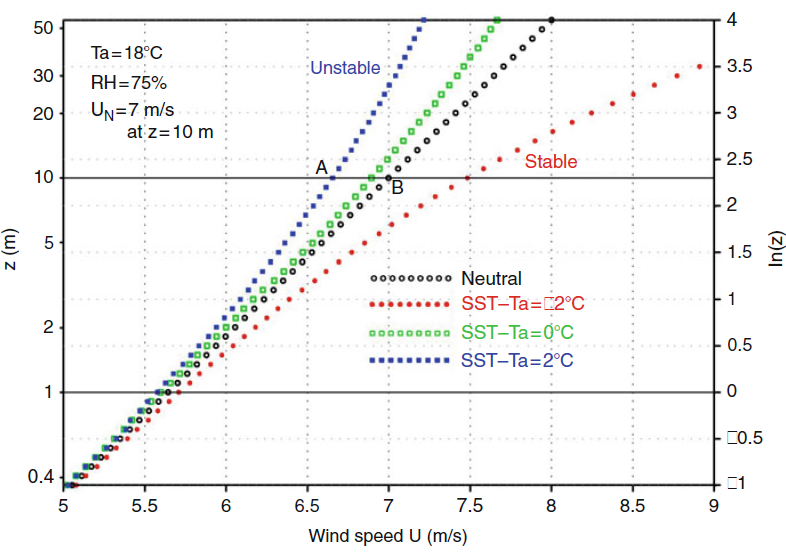
\includegraphics[width=0.75\linewidth]{Figures/Chapter2/stability.png}
%\decoRule
\caption{The influence of the neutral stability assumption in various conditions and heights near the sea surface. Point B represents the wind speed at 10 meters under neutrally stable conditions and A the measured value. Derived from: \cite{Liu2014}}
\label{fig:stability}
\end{figure}

We also define the drag coefficient at 10 meters height for a neutrally stable atmospheric boundary layer using \ref{eqn:cd_non_neutral}:


\begin{equation}
C_{DN10} = \left( \frac{k}{\ln{\left( 10/z_{0} \right)}} \right)^2
\label{eqn:cd_neutral}
\end{equation}

In this case, it is evident that estimating $C_{D}$ means that we can estimate the $z_{0}$. The roughness length over the ocean is not constant and dependent on the sea state. There are proposed methodologies to predict the roughness length from the wave age and SWH \cite{Taylor2001}. An extensive literature review of the most popular drag coefficient and roughness length parameterizations is available in the literature \cite{Bryant2016, Zhao2019}. The latter also explores the parameterization of $C_{D}$ and $z_{0}$ using the wave age and the wave steepness ($H/\lambda$). As the surface wind increases until the ocean surface gets fully rough, the wind stress strengthens its impact, and $C_{D}$ has higher values. Although it is true for moderate to high winds, it has been proven that the linear increase of the drag coefficient with increased wind speed does not apply for low wind speeds.  During conditions of very low winds ($u_{10} < 4 m/s$)  and the presence of aligned with the wind direction swells, the momentum flux reserves its sign from positive to negative, and the assumption of a neutrally stable, logarithmic profile over the sea surface is no longer valid \cite{Edson2013, Grachev2001, Hanley2008}.

From the number of available parameterizations, it is evident that the task to describe the air-sea interactions sufficiently is multi-faceted. This study uses a specific parameterization while considering the errors therein and the possible deviations from the truth. Specifically, we use equation \ref{eqn:u10} to adjust the reported wind speed observations from the buoys to the reference height of 10 meters. Representative values of $C_{D} = 1.2 \times 10^{-3}$ and the corresponding $z_{0} = 9.7 \times 10^{-5} m$ derived from \ref{eqn:cd_neutral} are also used in similar studies \cite{Ribal2019, Young2017}. Anemometers onboard buoys are placed on various heights (3.5 to 4.5 meters) depending on the buoy type. Hence, adjusting to a reference height is also beneficial for consistent comparisons.



%----------------------------------------------------------------------------------------


\section{Literature  review  of  bulk  formulae  for  wind-wave  relationships}\label{wind_wave_relationships}


In the first section of this Chapter \ref{swh_spectra}, we showed that SWH is estimated from the frequency spectrum and it is equal to four times the integral of the area under the continuous line of the spectrum, or the RMS elevation.

Historically, WS and SWH relationships are synonymous to the wave spectrum. Pierson's spectrum approach to ocean waves \cite{Pierson1955} was transcedental as he developed the theoretical background and the statistics of ocean wave spectra. Neumann implemented Pierson's theory and created the first wave spectrum using visual wave observations from ships. The Neumann spectrum was the first to connect the WS at the height of the anemometer as a driving force for the waves with the frequency spectrum. The fully developed or fully aroused sea was then defined as the sea state with a spectrum of all frequency components with the maximum energy under a specific value of WS forcing. This led to the SWH definition and the first relationships of SWH and WS based on the wave spectrum of a fully developed sea. The first three relationships came from the Pierson-Neumann system of equations \ref{eqn:pierson_neumann}, the  Sverdrup-Munk-Bretschneider wave forecasting method \ref{eqn:sverdrup_munk} and the Darbyshire spectrum \ref{eqn:darbyshire}. 

\begin{equation}
H_{s} = 7.065 \times 10^{-6} u^{2.5}
\label{eqn:pierson_neumann}
\end{equation}

\begin{equation}
H_{s} = 2.667 \times 10^{-4} u^{2}
\label{eqn:sverdrup_munk}
\end{equation}

\begin{equation}
H_{s} = 1.39 \times 10^{-4} u^{2}
\label{eqn:darbyshire}
\end{equation}

A comparison of theoretical spectra and their corresponding wind-wave relationships is available in \cite{Neumann1957}.

Kitagorodskii based on the Pierson-Moskowitz spectrum \cite{Pierson1964}, proposed similar empirical laws for the fully-developed sea. One of Kitagorodskii's empirical formulas is also the wave age wind-wave equilibrium equation \ref{eqn:wave_age}. For the fully-developed sea, he connected $u_{10}$ with $H_{s}$ \cite{CsanadyASI2001}:

\begin{equation}
H_{s} = \frac{0.2}{g} u_{10}^{2}
\label{eqn:kitagorodskii}
\end{equation}

A few years later, Carter \cite{Carter1982} reviewed the JONSWAP spectrum \cite{Hasselmann1973} and proposed the following relationship:

\begin{equation}
H_{s} = 0.02466 u_{10}^{2}
\label{eqn:jonswap}
\end{equation}

This relationship is also used as a reference in similar and contemporary studies \cite{Andreas2007}. Carter also proposed equations for the duration and fetch-limited seas:

\begin{equation}
H_{s} = 0.0163 X^{0.5} u_{10}
\label{eqn:fetch_limited}
\end{equation}

\begin{equation}
H_{s} = 0.0146 D^{5/7} u_{10}^{9/7}
\label{eqn:duration_limited}
\end{equation}

The sea is considered duration-limited when:

\begin{equation}
D > 1.167 X^{0.7} u_{10}^{-0.4}
\label{eqn:duration_limited_condition}
\end{equation}

\emph{X} is the fetch, the perpendicular distance to the upwind coast in kilometers and \emph{D} is the duration in hours. In this study, fetch is not included directly in the estimations. However, we examine the relationships for each of the main wind directions to indirectly connect them with the variation of the fetch in coastal regions.

WMO \cite{Organization1998a} suggests a similar empirical relationship for the estimation of SWH when $u_{10}$ is given.

\begin{equation}
H_{s} = \left(\frac{u_{10}}{12.5}\right)^{2}
\label{eqn:wmo_relationship}
\end{equation}

Finally, other studies incorporate wind-wave relationships from wave models for classification of the sea state into wind-waves and swells using altimeter data \cite{Chen2002}.

All the relationships mentioned above are valid under the assumptions of deep water waves and fully developed seas. Consequently, SWH cannot be accurately estimated from $u_{10}$ in all other growth stages or with presence of swells. 



%----------------------------------------------------------------------------------------


\section{Wind Speed Probability Density Functions}\label{wind_wave_pdfs}


This section is about the statistical interpretation of the long-term time series from the buoys. Specifically, the ultimate goal is to indicate the Probability Density Functions (PDF) that describe the $u_{10}$ distribution as it is estimated from the buoy records for each location.

Wind PDFs are required for design assessment at the offshore wind farm site before its installation \cite{Commision2019}. They are an integral part of the wind data analysis, and they are usually combined with the wind roses that provide the directional distribution of the wind speed \cite{DNVGL2018}. The average wind turbine
power is also associated with the PDF estimation \cite{Morgan2011}. For the wind PDF estimation, the suggested buoy dataset is the 10-minute average $U_{10}$. Although the modern wind turbine hub heights are greater than or equal to 100 meters, an extrapolation of the surface WS to such height would result in high uncertainty \cite{Ng2016}. Therefore, a reference height of 10 meters is selected for this study. The results would also prove useful as a reference to a similar estimation of the PDFs from wind lidar buoy and offshore wind tower observations in a later stage.

The standard and most widely-accepted wind speed distribution is the Weibull:


\begin{equation}
f(x) = \alpha x^{\alpha-1} exp\left( - x^\alpha \right)
\label{eqn:weibull_2p}
\end{equation}

Where $\alpha>0$ is the shape parameter. The best fit to our data is the 3-parameter Weibull though, for $y = (x-\gamma)/\eta$, where $\eta$ is the scale and $\gamma$ is the location parameter. Special cases of the Weibull are the Exponential ($\beta = 1$) and the Rayleigh ($\alpha = 2$) distributions.

There also regional characteristics of the wind speed distribution. Previous studies using buoy data have proved that the Weibull distribution is adequate for estimating the surface wind PDFs only for specific regions \citep{Morgan2011}. They propose that universal models should be a mixture of multiple distributions with different assigned weights for each distribution, depending on the domain. There are also studies suggesting that the Johnson $S_{B}$ \cite{Soukissian2013, Soukissian2014} distribution can be accepted as an alternative PDF and the best fit for certain regions. As described in the results, we identify and evaluate four distribution with the best fit for the WS data in SNE. Two of them, Weibull and Rayleigh are already referenced above. Besides, the Beta and Johnson $S_{B}$ distributions are also suggested to describe the long-term WS distribution at SNE:


\begin{equation}
f(x) = \frac{\Gamma\left(\alpha+\beta\right)}{\Gamma(\alpha)\Gamma(\beta)} x^{\alpha-1}(1-x)^{\beta-1}
\label{eqn:beta}
\end{equation}

This is the Beta 2P distribution where $\Gamma$ is the Gamma function and $\alpha > 0$, $\beta > 0$ are the shape parameters. We evaluate the 4P Beta PDF by adding scale and location parameters for $y = (x-\gamma)/\eta$, where $\eta$ is the scale and $\gamma$ is the location parameter respectively.


\begin{equation}
f(x) = \frac{b}{x(1-x)} \phi\left(\alpha+\beta\log{\frac{x}{1-x}}\right)
\label{eqn:johnsonsb}
\end{equation}


This is the Johnson $S_{B}$ 2P distribution where $\alpha > 0$, $\beta > 0$ are the shape parameters and $\phi$ is the normal distribution PDF. We evaluate the 4P Johnson $S_{B}$ PDF by adding a scale and location parameters for $y = (x-\gamma)/\eta$, where $\eta$ is the scale and $\gamma$ is the location parameter respectively.


We identify the single, univariate distributions of best fit to the long-term $u_{10}$ time series using the extended \emph{SciPy} library of PDFs for each buoy location. This library utilizes the Maximum Likelihood Estimation (MLE) methodology for fitting to the theoretical distributions and the estimation of the distribution parameters.


%----------------------------------------------------------------------------------------



\section{Principles of Satellite Altimetry}\label{AltimetryPrinciples}

The Radar altimeter is an active, nadir looking microwave instrument that emits its impulses to the earth's surface. Once it receives them back, it measures the travel time, the magnitude, and the shape of each return signal.

The average of hundreds of pulses shape the mean returned signal. Specifically, the signals tracked originally by the altimeter are convolved to a single waveform after being fitted to a mathematical model. These function fitting methods are evolving through the years and are described in \cite{Gommenginger2011}. The process is fundamental for satellite altimetry and constitutes the retracking model. The mathematical model used for the fitting of the retracking algorithm is the Brown-Hayne model \cite{Brown1977TheApplications, Hayne1980RadarScattering} for the Low-Resolution Mode (LRM) and the SAMOSA model for the Synthetic Aperture Radar (SAR) altimetry \citep{Ray2015SARModel}. As a result, a typical waveform in the open ocean has three distinct areas, as presented in Figure~\ref{fig:altimeter_waveform}. The first one is the area of low, close to zero power. The second is the leading edge, which contains the area from the time that the waveform's power begins to increase until its peak. The third is the trailing edge, which is the area of decaying power of the waveform.

Except for the impulses' signal, an accurate determination of the earth's orbit is critical, especially the radial component. In addition, the target accuracy of the distance between the satellite and the sea level is on the order of 1 centimeter. Therefore, corrections due to the errors caused by the signal's delay as it travels through the ionosphere and the atmosphere have to be applied. The ionospheric corrections are essential to measuring the delay of the altimeter signal's travel time caused by the ionosphere's free electrons. It is also one reasons why a dual-frequency (Ku or Ka and C band) altimeter instrument is needed onboard the satellite. Besides, there are two kinds of atmospheric corrections: the dry tropospheric and the wet tropospheric correction. For the latter, the microwave radiometer instrument is used to measure the water vapor in the atmosphere. A significant challenge for coastal altimetry is that the microwave radiometer footprint radius is close to 50 kilometers. Therefore, the brightness temperature of the land contaminates the measurement in coastal areas. The wet troposphere correction is also very challenging due to the spatiotemporal variability of water vapor in the atmosphere. For these reasons, the uncontaminated signal in the open ocean is used in conjunction with in situ observations, when and where available, to correct the wet troposphere delay. Furthermore, there is uncertainty also at the surface of the ocean. Specifically, geophysical adjustments have to be applied to estimate parameters such as the earth and ocean tides, the sea state bias, and a dynamic atmosphere correction.

In coastal altimetry, the retracking model's fitting to get the final waveform has additional challenges as we get closer to the coast. Due to the extended radius of the altimeter footprint, land intrudes in the received signal, and there is land contamination of the waveform \citep{Halimi2013}. Hence, the final waveform can be corrupted, especially in high sea state conditions. Secondly, as we get closer to the coast, the footprint's backscatter is different from the one in the open ocean. Indeed, in coastal areas, the altimeter footprint may cover both a windy area with considerable sea surface roughness and an area of calm sea state with an almost flat surface “shaded” by the wind. As a result of the limitations mentioned above, the final waveform shows unusually higher power peaks in the trailing edge, a part of the waveform that we should otherwise not consider when fitting to the model to estimate the geophysical parameters.


\begin{figure}[H]
\centering
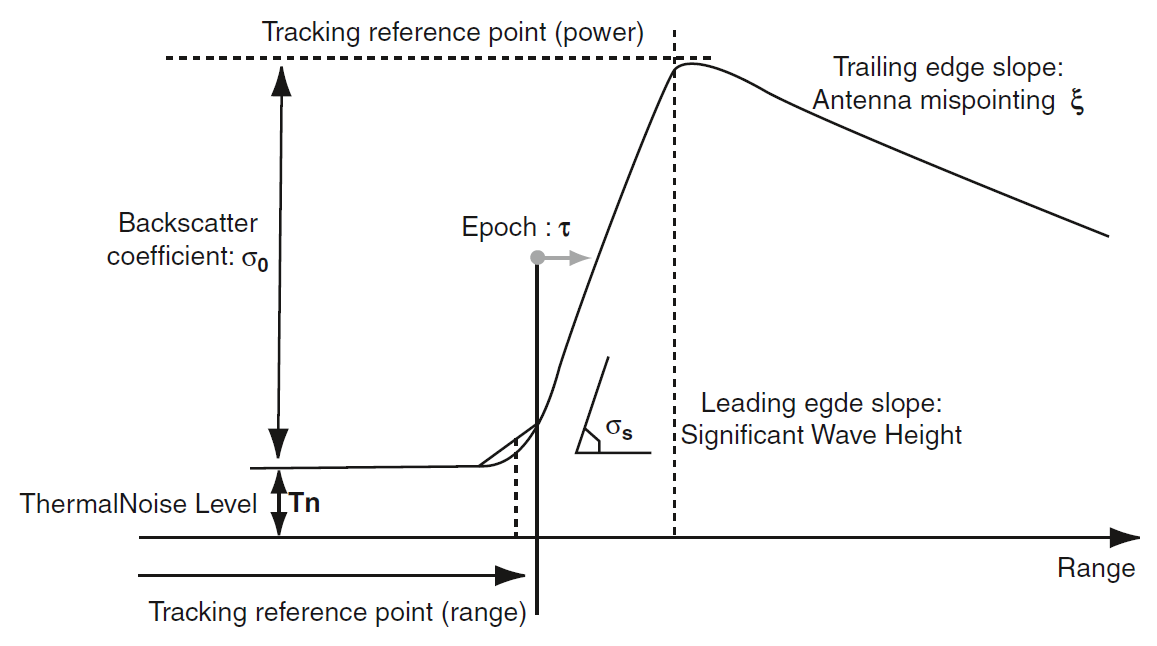
\includegraphics[width=0.85\linewidth]{Figures/Chapter2/altimeter_waveform.png}
%\decoRule
\caption{The Brown theoretical retracking model for LRM altimetry and the derived parameters. Derived from: \cite{Gommenginger2011}.}
\label{fig:altimeter_waveform}
\end{figure}



These limitations are evident when we consider the pulse-limited signal of the LRM altimeters. The effective footprint of the LRM altimeter is given by:

\begin{equation}
f = \frac{\pi R_{0} (c\tau + 2 H_{s})}{1 + R_{0}/R_{E}}
\label{eqn:effective_footprint}
\end{equation}

Where \emph{c} is the speed of light, \emph{$\tau$} is the pulse length, $H_{s}$ the SWH, $R_{0}$ the altitude of the satellite and $R_{E}$ the Earth's radius.

When the sea is calm, the altimeter's footprint is approximately a 2-kilometer radius in both directions, the along-track and the across-track. In contrast, during a storm or high sea state, the effective footprint can extend to over 7 kilometers. The principles of pulse-limited altimetry are extensively described in \cite{Chelton2001}. SAR or delay-Doppler altimetry using the Ray et al. \cite{Ray2015SARModel} model, revolutionized how the signal's power is used. On the one hand, it considers both the leading and the trailing edge of the retracked waveform instead of the smaller area of the leading edge considered for the LRM. The finer resolution on the along-track and the waveform's reduced noise are the main aspects of the evolution of SAR altimetry \cite{KeithRaney1998}. Its Pulse-Doppler-limited footprint's resolution can be constrained to approximately 300 meters only on the along-track. On the across-track, though, the resolution remains similar to the pulse-limited LRM. The effective footprint of SAR looks like slices of the LRM circular footprint as in Figure~\ref{fig:SAR_LRM}. The SAR altimetry pioneer is Cryosat 2 satellite, as it is equipped with the SIRAL instrument that operates in both modes (see \ref{altimeter_data}). Raynal et al. \cite{Raynal2018} demonstrates the increased accuracy of the SAR's higher spatial resolution over different areas worldwide. The European Space Agency (ESA) Sentinel 3 twin satellites, A and B, are the first missions that use the SAR altimetry mode exclusively. Currently, the remaining altimeters in orbit are operating in LRM mode. On the other hand, SARAL-AltiKa is the only LRM altimeter that emits its impulses in higher frequency using the Ka-band, which increases the accuracy of the measured parameters and reduces the noise of the final waveform.


 
\begin{figure}[H]
\centering
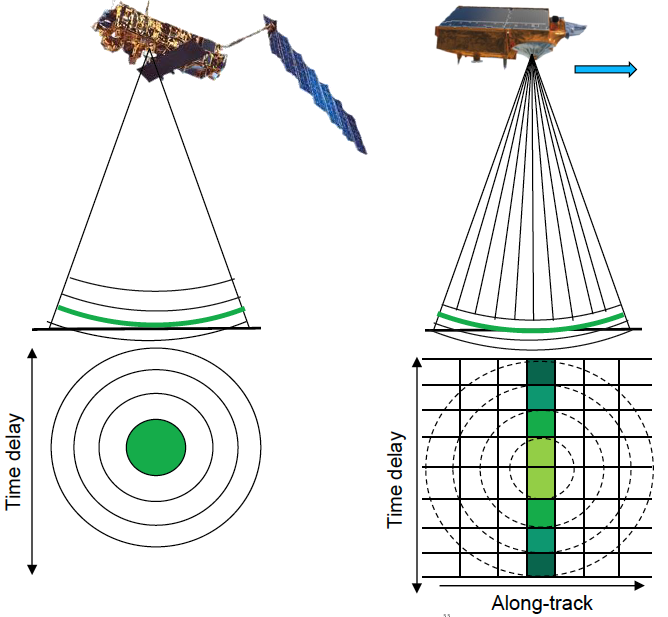
\includegraphics[width=0.8\linewidth]{Figures/Chapter2/sar_vs_lrm.png}
%\decoRule
\caption{A representation of the LRM and SAR altimeter footprint.}
\label{fig:SAR_LRM}
\end{figure}


We can determine at least three essential parameters from the retracked waveform \ref{fig:altimeter_waveform}. The first one is the epoch. We can then estimate the range from the epoch, which is the signal's travel time, until it reaches back the satellite and is connected with the Sea Surface Height (SSH). The second important parameter of the waveform is the slope of the leading edge (or width or rising time of the leading edge), which is connected to the estimation of the SWH. The third essential parameter is the backscatter coefficient derived by the received signal's power and is associated with the surface WS. For this study, the focus is on two of the three aforementioned geophysical parameters and their corresponding estimates, namely the SWH and the WS.

As previously discussed, the estimation of the SWH is connected with the slope of the leading edge. Specifically, the slope is a function of the root mean square error of the SWH. A steep leading edge represents a small value of the SWH. In contrast, for higher values of SWH, for example, during a storm, the return signal starts to rise earlier until it reaches its peak power, and also, the shape of the echo is different \cite{Ardhuin2019}. The difference between the two resulting waveforms, one during a calm sea and one for a rougher sea surface, is shown in Figure~\ref{fig:swh_altimeter}(b). It is evident that SWH from altimeters is derived with an entirely different measurement method with respect to buoys described in Chapter~\ref{swh_spectra}.


The radar altimeter also measures the backscatter signal's strength. This value is inversely proportional to the sea surface Mean Square Slope (MSS) \cite{Cox1954} which is related to the sea surface roughness induced by the wind. Therefore, the estimated WS increases as the surface MSS gets higher and the backscatter becomes smaller. The main source of errors in the altimeter estimation of the WS is the empirical nature of the corresponding algorithms that do not consider the impact of the sea state growth, primarily due to swells \cite{Abdalla2007, Glazman1990}. The retracking of hundreds of noisy signals and the need for reliable atmospheric corrections, notably close to the coast, makes the task even more challenging.



\begin{figure}[H]
\centering
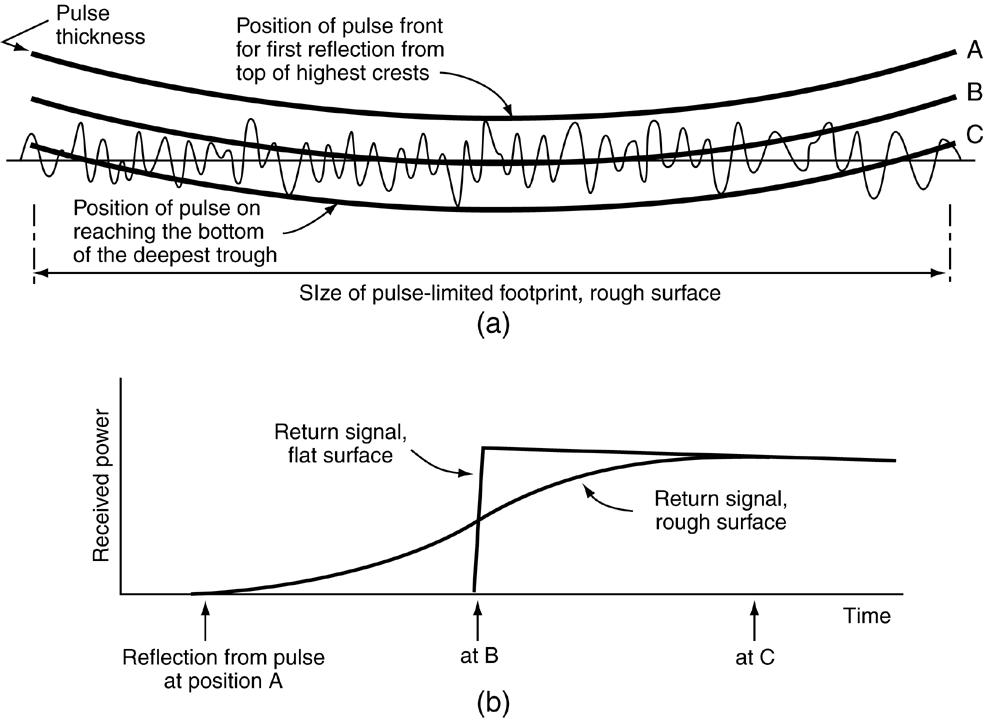
\includegraphics[width=0.8\linewidth]{Figures/Chapter2/swh_altimeter.png}
%\decoRule
\caption{(a) Illuminated surface geometry. (b) The resulting shape of the reflected pulse. Derived from: \citep{Robinson2010}}
\label{fig:swh_altimeter}
\end{figure}






%----------------------------------------------------------------------------------------



